% Font options: 10pm, 11pt, 12pt
% Align headings left instead of center: nocenter
\documentclass[xcolor=x11names,compress]{beamer}\usepackage[]{graphicx}\usepackage[]{color}
%% maxwidth is the original width if it is less than linewidth
%% otherwise use linewidth (to make sure the graphics do not exceed the margin)
\makeatletter
\def\maxwidth{ %
  \ifdim\Gin@nat@width>\linewidth
    \linewidth
  \else
    \Gin@nat@width
  \fi
}
\makeatother

\definecolor{fgcolor}{rgb}{0.345, 0.345, 0.345}
\newcommand{\hlnum}[1]{\textcolor[rgb]{0.686,0.059,0.569}{#1}}%
\newcommand{\hlstr}[1]{\textcolor[rgb]{0.192,0.494,0.8}{#1}}%
\newcommand{\hlcom}[1]{\textcolor[rgb]{0.678,0.584,0.686}{\textit{#1}}}%
\newcommand{\hlopt}[1]{\textcolor[rgb]{0,0,0}{#1}}%
\newcommand{\hlstd}[1]{\textcolor[rgb]{0.345,0.345,0.345}{#1}}%
\newcommand{\hlkwa}[1]{\textcolor[rgb]{0.161,0.373,0.58}{\textbf{#1}}}%
\newcommand{\hlkwb}[1]{\textcolor[rgb]{0.69,0.353,0.396}{#1}}%
\newcommand{\hlkwc}[1]{\textcolor[rgb]{0.333,0.667,0.333}{#1}}%
\newcommand{\hlkwd}[1]{\textcolor[rgb]{0.737,0.353,0.396}{\textbf{#1}}}%
\let\hlipl\hlkwb

\usepackage{framed}
\makeatletter
\newenvironment{kframe}{%
 \def\at@end@of@kframe{}%
 \ifinner\ifhmode%
  \def\at@end@of@kframe{\end{minipage}}%
  \begin{minipage}{\columnwidth}%
 \fi\fi%
 \def\FrameCommand##1{\hskip\@totalleftmargin \hskip-\fboxsep
 \colorbox{shadecolor}{##1}\hskip-\fboxsep
     % There is no \\@totalrightmargin, so:
     \hskip-\linewidth \hskip-\@totalleftmargin \hskip\columnwidth}%
 \MakeFramed {\advance\hsize-\width
   \@totalleftmargin\z@ \linewidth\hsize
   \@setminipage}}%
 {\par\unskip\endMakeFramed%
 \at@end@of@kframe}
\makeatother

\definecolor{shadecolor}{rgb}{.97, .97, .97}
\definecolor{messagecolor}{rgb}{0, 0, 0}
\definecolor{warningcolor}{rgb}{1, 0, 1}
\definecolor{errorcolor}{rgb}{1, 0, 0}
\newenvironment{knitrout}{}{} % an empty environment to be redefined in TeX

\usepackage{alltt}
%\documentclass[xcolor=x11names,compress,handout]{beamer}
\usepackage[]{graphicx}
\usepackage[]{color}
\usepackage{booktabs}
\usepackage{hyperref}
\usepackage{tikz}
\usepackage{multirow}
\usepackage{dcolumn}
\usepackage{bigstrut}
\usepackage{amsmath} 
\usepackage{xcolor,colortbl}
\usepackage{amssymb}
%\newcommand{\done}{\cellcolor{teal}#1}

%% Beamer Layout %%%%%%%%%%%%%%%%%%%%%%%%%%%%%%%%%%
\useoutertheme[subsection=false,shadow]{miniframes}
\useinnertheme{default}
\usefonttheme{serif}
\usepackage{Arev}
\usepackage{pdfpages}

\setbeamerfont{title like}{shape=\scshape}
\setbeamerfont{frametitle}{shape=\scshape, size=\normalsize}

\definecolor{dkblue}{RGB}{0,0,102}

\setbeamercolor*{lower separation line head}{bg=dkblue} 
\setbeamercolor*{normal text}{fg=black,bg=white} 
\setbeamercolor*{alerted text}{fg=red} 
\setbeamercolor*{example text}{fg=black} 
\setbeamercolor*{structure}{fg=black} 
 
\setbeamercolor*{palette tertiary}{fg=black,bg=black!10} 
\setbeamercolor*{palette quaternary}{fg=black,bg=black!10} 

\renewcommand{\(}{\begin{columns}}
\renewcommand{\)}{\end{columns}}
\newcommand{\<}[1]{\begin{column}{#1}}
\renewcommand{\>}{\end{column}}

\AtBeginSection{\frame{\sectionpage}}
\usepackage{xcolor}
\hypersetup{
    colorlinks,
    linkcolor={red!50!black},
    citecolor={blue!50!black},
    urlcolor={blue!80!black}
}

\setbeamertemplate{navigation symbols}{} 
\setbeamertemplate{footline}[frame number]
\setbeamertemplate{caption}{\raggedright\insertcaption\par}

\setbeamersize{text margin left=5pt,text margin right=5pt}

%%%%%%%%%%%%%%%%%%%%%%%%%%%%%%%%%%%%%%%%%%%%%%%%%%


\title{FLS 6441 - Methods III: Explanation and Causation}
\subtitle{Week 7 - Discontinuities}
\author{Jonathan Phillips}
\date{May 2019}
\IfFileExists{upquote.sty}{\usepackage{upquote}}{}
\begin{document}




\frame{\titlepage}

\begin{frame}
\frametitle{Classification of Research Designs}
\footnotesize
\begin{table}[htbp]
  \centering
  \scalebox{0.7}{
    \begin{tabular}{|p{2.2cm}|p{5cm}|c|c|}
    \hline
          &       & \multicolumn{1}{p{2.4cm}|}{\textbf{Independence of Treatment Assignment}} & \multicolumn{1}{p{3cm}|}{\textbf{Researcher Controls Treatment Assignment?}} \bigstrut\\
    \hline
    \multicolumn{1}{|p{2.9cm}|}{\multirow{2}[4]{2.9cm}{\textbf{Controlled Experiments}}} & Field Experiments & \checkmark      & \checkmark  \bigstrut\\
\cline{2-4}          & Survey and Lab Experiments &  \checkmark     & \checkmark \bigstrut\\
    \hline
          &       &       &  \bigstrut\\
    \hline
    \multicolumn{1}{|p{2.9cm}|}{\multirow{3}[6]{2.9cm}{\textbf{Natural Experiments}}} & Natural Experiments &  \checkmark     &  \bigstrut\\
\cline{2-4}          & Instrumental Variables & \checkmark      &  \bigstrut\\
\cline{2-4}          & Discontinuities & \checkmark      &  \bigstrut\\
    \hline
          &       &       &  \bigstrut\\
    \hline
    \multicolumn{1}{|p{2.9cm}|}{\multirow{4}[8]{2.9cm}{\textbf{Observational Studies}}} & Difference-in-Differences &       &  \bigstrut\\
\cline{2-4}          & Controlling for Confounding &       &  \bigstrut\\
\cline{2-4}          & Matching &       &  \bigstrut\\
\cline{2-4}          & Comparative Cases and Process Tracing &       &  \bigstrut\\
    \hline
    \end{tabular}}%
  \label{tab:addlabel}%
\end{table}%
\normalsize
\end{frame}


\section{Discontinuities}

\begin{frame}
\frametitle{Discontinuities}
\begin{itemize}
\item Natural Experiments
\pause
\item Where the 'as-if' random treatment assignment comes from \textit{discontinuities} in rules
\pause
\begin{itemize}
\item Rules that \textbf{treat very similar people very differently}
\pause
\item Small differences on a \textbf{continuous} variable create big differences on a \textbf{binary treatment} variable
\end{itemize}
\end{itemize}
\end{frame}

\begin{frame}
\frametitle{Discontinuities}
\begin{center}
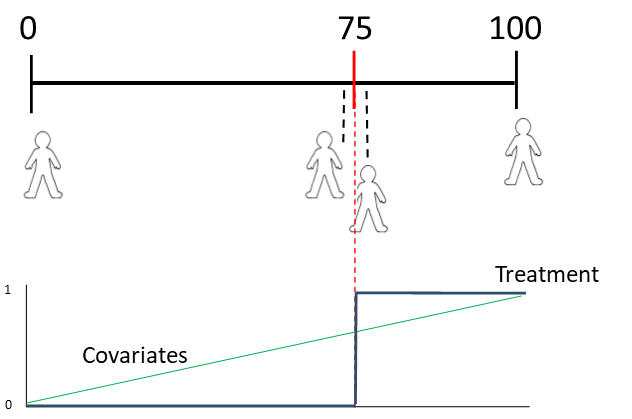
\includegraphics[scale=0.55]{Scale.png}
\end{center}
\end{frame}


\begin{frame}
\frametitle{Discontinuities}
\begin{itemize}
\item Example thresholds:
\begin{itemize}
\item Exam cutoffs
\item Age cutoffs
\item Policy eligibility rules
\item Close elections
\item Adminsitrative boundaries
\end{itemize}
\end{itemize}
\end{frame}

\begin{frame}
\frametitle{Discontinuities}
\begin{itemize}
\item Why do discontinuities assign treatment 'as-if' random?
\pause
\item Maybe they don't! \pause It depends on how much \textbf{control} people have over their 'scores'
\pause
\begin{itemize}
\item Could you get a score of exactly 10 in naming all the Brazilian states?
\pause
\item Could you get a score of exactly 150 on the GRE?
\end{itemize}
\pause
\item We need qualitative evidence that people cannot 'choose' their score perfectly
\pause
\item Then the factors that influence \textit{small} changes in score should be independent of potential outcomes
\pause
\begin{itemize}
\item Weather
\item Chance
\item Mistakes
\end{itemize}
\end{itemize}
\end{frame}

\begin{frame}
\frametitle{Discontinuities}
\begin{itemize}
\item Regression Discontinuity
\begin{itemize}
\item What is the Treatment Assignment Mechanism?
\pause
\[
D_i=
\begin{cases}
1 & \text{if }x_i \geq \bar{x} \\
0 & \text{if }x_i < \bar{x}
\end{cases}
\]
\pause
\item 'As-if' random only \textbf{really close to the threshold}
\pause
\item For units just above and below the threshold:
\begin{itemize}
\item Their potential outcomes are almost the same
\pause
\item Their covariates are almost the same
\pause
\item They are plausible counterfactuals for each other
\end{itemize}
\end{itemize}
\end{itemize}
\end{frame}


\begin{frame}
\frametitle{Discontinuities}
\begin{itemize}
\item Comparisons in a regression discontinuity are always \textit{imperfect}
\pause
\item \textbf{Field experiment:} For every value of $X$ we have both treated and control values
\pause
\item \textbf{Discontinuity:} We \textbf{cannot} have treated and control values with the same value of the running variable $x$
\pause
\item So we have to \textbf{extrapolate} to guess what the potential outcomes would be if unit $i$ was treated instead of control
\pause
\item So we need more assumptions (and more N)!
\end{itemize}
\end{frame}

\begin{frame}
\frametitle{Discontinuities}
\begin{knitrout}
\definecolor{shadecolor}{rgb}{0.969, 0.969, 0.969}\color{fgcolor}
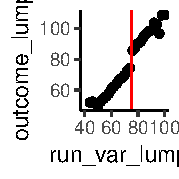
\includegraphics[width=\maxwidth]{figure/chart2_binned-1} 

\end{knitrout}
\end{frame}


\begin{frame}
\frametitle{Discontinuities}
\begin{itemize}
\item Regresssion Discontinuity Variables:
\begin{itemize}
\item \textbf{Running Variable $x_i$:} The \textit{continuous} variable to which the threshold/cutoff is applied, eg. exam score
\pause
\item \textbf{Treatment $D_i$:} Binary 0/1 depending on whether the running variable is above or below the threshold ($x_i>=\bar{x}$)
\pause
\item \textbf{Outcome $Y_i$:} Any subsequent outcome you have measured
\end{itemize}
\end{itemize}
\end{frame}

\begin{frame}
\frametitle{Discontinuities}
\begin{itemize}
\item Regression Discontinuity Assumptions:
\begin{enumerate}
\item Potential outcomes vary continuously (are independent of treatment) \textbf{at} the threshold
\begin{enumerate}
\pause
\item Units cannot precisely control their score and sort either side of the threshold
\pause
\item The threshold is not chosen strategically
\end{enumerate}
\pause
\item No compound treatments
\pause
\item No spillovers (SUTVA)
\end{enumerate}
\end{itemize}
\end{frame}

\begin{frame}
\frametitle{Discontinuities}
\begin{itemize}
\item The threshold is more likely to be independent of potential outcomes if:
\pause
\begin{itemize}
\item Units are not aware of the threshold
\pause
\item The threshold is decided after units make choices
\pause
\item The running variable is hard to manipulate precisely
\pause
\item The threshold is chosen before scores are known
\pause
\end{itemize}
\item We need qualitative evidence to support these assumptions
\end{itemize}
\end{frame}

\begin{frame}
\frametitle{Discontinuities}
\begin{itemize}
\item We can check for sorting with a density test
\item If units are bunched just above the threshold, this suggests manipulation
\end{itemize}

\end{frame}


\section{Estimating Regression Discontinuities}

\begin{frame}
\frametitle{Estimating Discontinuities}
\begin{itemize}
\item 3 Regression Discontinuity Methodologies:
\begin{enumerate}
\item \textbf{Difference-in-means:} Define a small window either side of the threshold and compare average outcomes in this window
\begin{itemize}
\item Can be biased since we're ignoring the omitted variable effect of the running variable on the outcome
\pause
\end{itemize}
\item \textbf{'Full data' regression discontinuity:} Uses \textit{all} the data:
$$Y_i = \alpha + \beta_1 Running\_Variable_i + \beta_2 Treatment_i + \epsilon_i$$
\begin{itemize}
\item Controls for the 'smooth' variation in the running variable
\item Estimates the 'jump' impact of treatment with a binary variable (dummy)
\pause
\end{itemize}
\item \textbf{'Limited-bandwidth' regression discontinuity:}  A regression only using only data close to the threshold
\begin{itemize}
\item What \textit{bandwidth} around the threshold do we use?
\end{itemize}
\end{enumerate}
\end{itemize}
\end{frame}


\begin{frame}
\frametitle{Raw Data}
\begin{center}
\begin{knitrout}
\definecolor{shadecolor}{rgb}{0.969, 0.969, 0.969}\color{fgcolor}
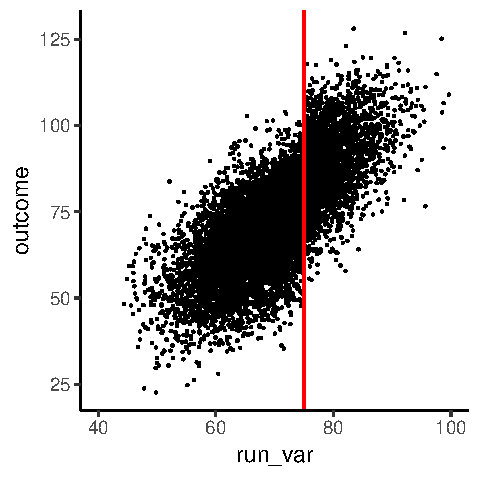
\includegraphics[width=\maxwidth]{figure/chart1-1} 

\end{knitrout}
\end{center}
\end{frame}

\begin{frame}
\frametitle{'Binned' Data}
\begin{center}
\begin{knitrout}
\definecolor{shadecolor}{rgb}{0.969, 0.969, 0.969}\color{fgcolor}
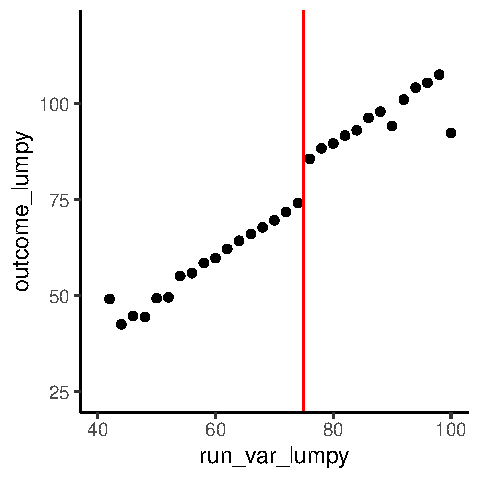
\includegraphics[width=\maxwidth]{figure/chart2-1} 

\end{knitrout}
\end{center}
\end{frame}

\begin{frame}
\frametitle{1. Difference-in-Means}
\begin{center}
\begin{knitrout}
\definecolor{shadecolor}{rgb}{0.969, 0.969, 0.969}\color{fgcolor}
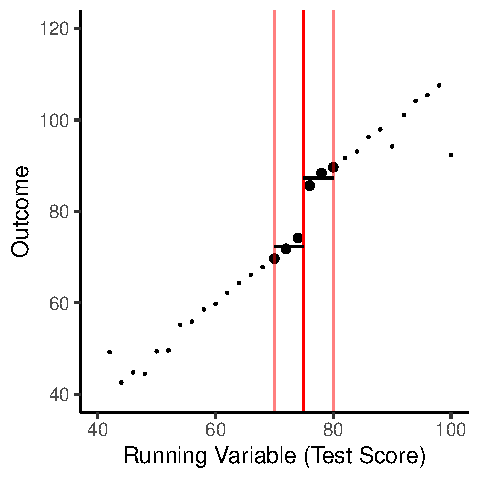
\includegraphics[width=\maxwidth]{figure/chart3-1} 

\end{knitrout}
\end{center}
\end{frame}

\begin{frame}
\frametitle{2. Full Data Regression - Linear}
\begin{center}
\begin{knitrout}
\definecolor{shadecolor}{rgb}{0.969, 0.969, 0.969}\color{fgcolor}
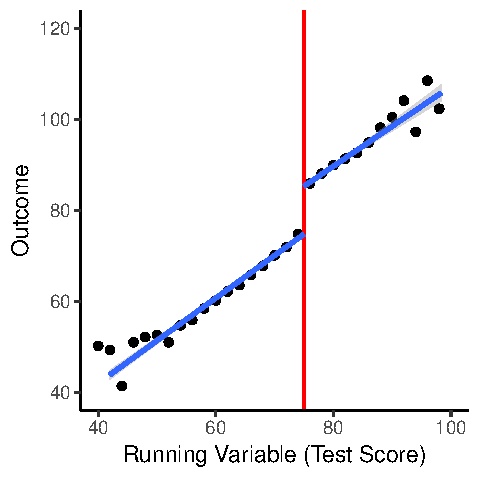
\includegraphics[width=\maxwidth]{figure/chart4-1} 

\end{knitrout}
\end{center}
\end{frame}

\begin{frame}
\frametitle{3. Limited-bandwidth Regression - Local Linear}
\begin{center}
\begin{knitrout}
\definecolor{shadecolor}{rgb}{0.969, 0.969, 0.969}\color{fgcolor}
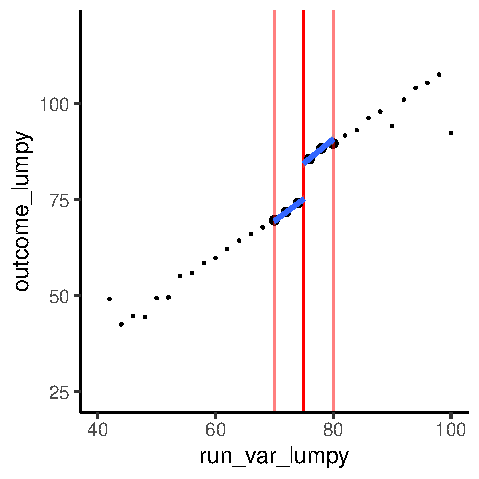
\includegraphics[width=\maxwidth]{figure/chart6-1} 

\end{knitrout}
\end{center}
\end{frame}

\begin{frame}
\frametitle{Estimating Discontinuities}
\begin{itemize}
\item Which method?
\pause
\begin{itemize}
\item Difference-in-means is probably biased, and we can easily do better
\pause
\item The full-data approach gives more precision but depends on the right model: linear, quadratic, etc., so more risk of bias
\pause
\item The combined approach uses less data (-precision) but is less dependent on the right model (-risk of bias)
\pause
\end{itemize}
\item In practice, apply all three as robustness checks
\end{itemize}
\end{frame}

\begin{frame}
\frametitle{2b. Full Data Regression - Non-linear}
\begin{center}
\begin{knitrout}
\definecolor{shadecolor}{rgb}{0.969, 0.969, 0.969}\color{fgcolor}
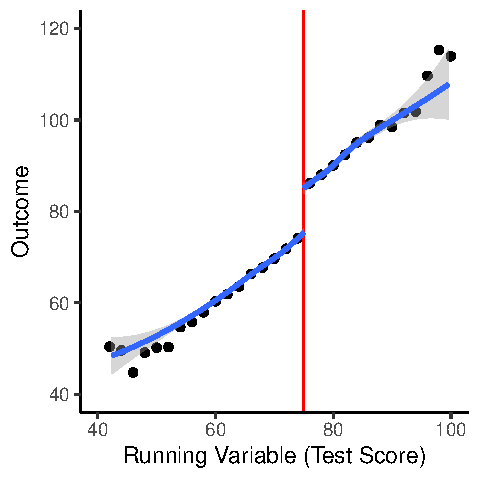
\includegraphics[width=\maxwidth]{figure/chart5-1} 

\end{knitrout}
\end{center}
\end{frame}


\begin{frame}
\frametitle{Estimating Discontinuities}
\begin{itemize}
\item Regression Discontinuity estimates a \textbf{Local Average Treatment Effect}
\pause
\begin{itemize}
\item Treatment assignment is only random at the threshold
\pause
\item Our estimates only apply to units close to the threshold
\pause
\item Units far from the threshold are very different for a reason, and causal effects are likely to be different
\end{itemize}
\end{itemize}
\end{frame}


\begin{frame}
\frametitle{Estimating Discontinuities}
\begin{itemize}
\item Limitations:
\begin{itemize}
\item Lots of alternative specifications so no single simple test
\pause
\item Less precise than a randomized trial, so we need more data
\pause
\item Risk of sorting/manipulation
\end{itemize}
\end{itemize}
\end{frame}

\section{Close Elections}

\begin{frame}
\frametitle{Close Elections}
\begin{itemize}
\item Close elections are one type of regression discontinuity in which political office is 'as-if' randomized
\pause
\item Useful for understanding the effects of political power
\pause
\begin{itemize}
\item \textbf{Running Variable: }Margin of victory
\item \textbf{Treatment: }Winning a close election
\item \textbf{Control: }Losing a close election
\item \textbf{Outcome: }Anything that happens later...
\end{itemize}
\end{itemize}
\end{frame}

\begin{frame}
\frametitle{Close Elections}
\begin{itemize}
\item How much faith should we have in 'close election' regression discontinuities?
\pause
\item Eggers et al (2013):
\pause
\begin{itemize}
\item US House of Representatives elections show sorting in very close elections (<1\%)
\pause
\item Politicians (incumbents, the wealthy) can control whether they win, even when it's a tight race
\pause
\item They have extremely detailed information to predict vote results
\pause
\item So potential outcomes are not balanced
\pause
\item But no other case (9 countries) has this problem
\end{itemize}
\end{itemize}
\end{frame}

\begin{frame}
\frametitle{Close Elections}
\begin{itemize}
\item Boas and Hidalgo (2011): How does incumbency affect control of the media?
\pause
\begin{itemize}
\item Radio licencing process depends on ability to lobby the Ministry and Congress
\pause
\item Local radio systematically used to favour specific politicians
\pause
\item Incumbents better placed to initiate exchange between Mayors and legislators
\pause
\end{itemize}
\item What is the challenge to causal inference here?
\end{itemize}
\end{frame}

\begin{frame}
\frametitle{Close Elections}
\begin{itemize}
\item \textbf{Population:} Brazilian councillors
\item \textbf{Sample:} Brazilian councillors in close elections that made radio licence applications in 2000/2004
\item \textbf{Running Variable:} Vote margin
\item \textbf{Treatment:} Just winning close election
\item \textbf{Control:} Just losing close election
\item \textbf{Treatment Assignment:} 'As-if' random in close elections
\item \textbf{Outcome:} Approved radio licence application rate
\end{itemize}
\end{frame}

\begin{frame}
\frametitle{Close Elections}
\begin{itemize}
\item Boas and Hidalgo (2011) Methodology:
\begin{enumerate}
\item Local Linear regression within bandwidth of 165 votes
\item Difference-in-Means within 10-40 vote bandwidth
\end{enumerate}
\end{itemize}
\end{frame}

\begin{frame}
\frametitle{Close Elections}
\begin{itemize}
\item Results
\begin{itemize}
\item Incumbent Vereadores are twice as likely (14-27 \% points) to have their radio licence applications approved
\end{itemize}
\end{itemize}
\end{frame}

\begin{frame}
\frametitle{Close Elections}
\begin{center}
\includegraphics[scale=0.33]{figure/BH_Results.png}
\end{center}
\end{frame}

\section{Geographic Discontinuities}

\begin{frame}
\frametitle{Geographic Discontinuities}
\begin{itemize}
\item What is the effect of programmatic governance reform on voters' attitudes?
\pause
\item Bihar is one of the poorest places on the planet and one of the worst goverened
\pause
\item \textbf{Before 2005:} 'Jungle raj': Clientelism, violence, corruption, caste bias
\pause
\item \textbf{After 2005:} Bihar is a programmatic reform success case
\pause
\end{itemize}
\end{frame}

\begin{frame}
\frametitle{Geographic Discontinuities}
\begin{figure}
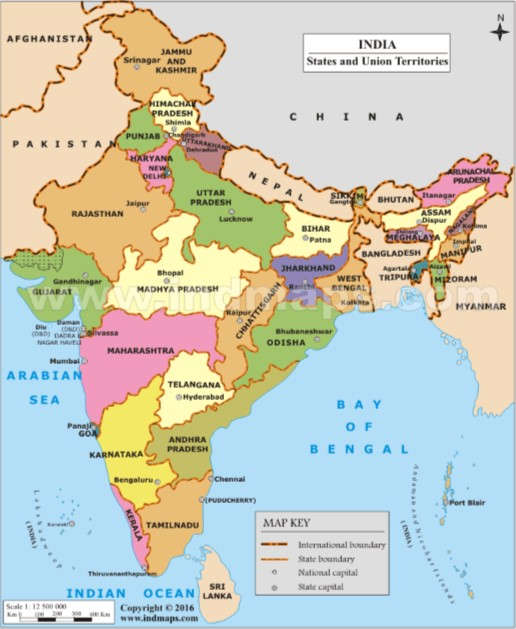
\includegraphics[scale=0.2]{figure/India_Map.jpg} 
\end{figure}
\end{frame}

\begin{frame}
\frametitle{Geographic Discontinuities}
\begin{itemize}
\item People in Jharkhand are plausible counterfactuals to people in Bihar because:
\pause
\begin{itemize}
\item Socioeconomic, geographic and national governance conditions are very similar at the border
\pause
\item Families have lived in their villages for decades
\pause
\item The two states were only created in 2001; before that they experienced the same relationship with government
\pause
\item The border was set according to old district borders, and not politically
\pause
\item Jharkhand did not experience the same governance improvements as Bihar
\end{itemize}
\end{itemize}
\end{frame}

\begin{frame}
\frametitle{Methodology}
\begin{itemize}
\item The 'running variable' is distance to the border, but in 2-dimensions:
\begin{multline}
y_i = \alpha + \beta Bihar_i + x_i + y_i \pause + x^2 + y^2 + x^3 + y^3 + x^4 + y^4 + x*y  \\+ x^2*y^2 + x^3*y^3 + x*y^2 + x*y^3 + x^2*y + x^3*y + \epsilon_i
\end{multline}
\item $\beta$ is our treatment effect of interest
\end{itemize}
\end{frame}

\begin{frame}
\frametitle{Geographic Discontinuities}
\begin{itemize}
\item Geographic Regression Discontinuity Design
\begin{itemize}
\item Exactly the same as a normal regression discontinuity, but in two dimensions (longitude and latitude)
\pause
\item \textbf{The Running Variable:} \pause Longitude and latitude
\pause 
\item \textbf{Treatment:} \pause Residents on the Bihar side of the border
\pause 
\item \textbf{Control:} \pause Residents on the Jharkhand side of the border
\pause 
\item \textbf{Treatment Assignment:} \pause State separation in 2001, Family history, and migration
\pause 
\item \textbf{Outcome:} \pause Political attitudes and behaviour
\end{itemize}
\end{itemize}
\end{frame}

\begin{frame}
\begin{figure}
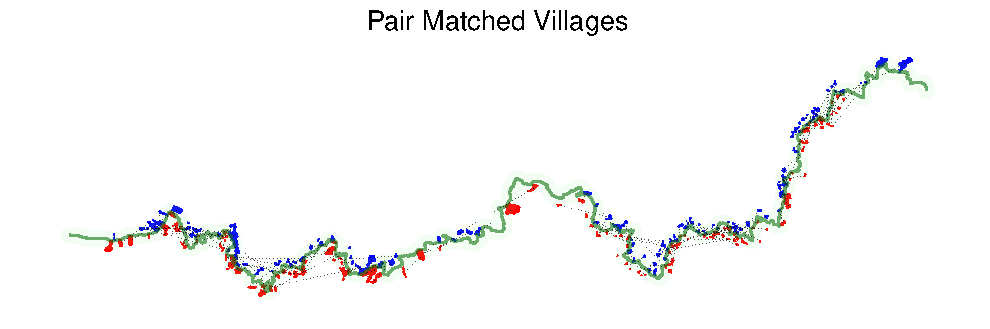
\includegraphics[width=\maxwidth]{figure/Map_Border-1.pdf}
\end{figure}
\end{frame}

\begin{frame}
\begin{figure}
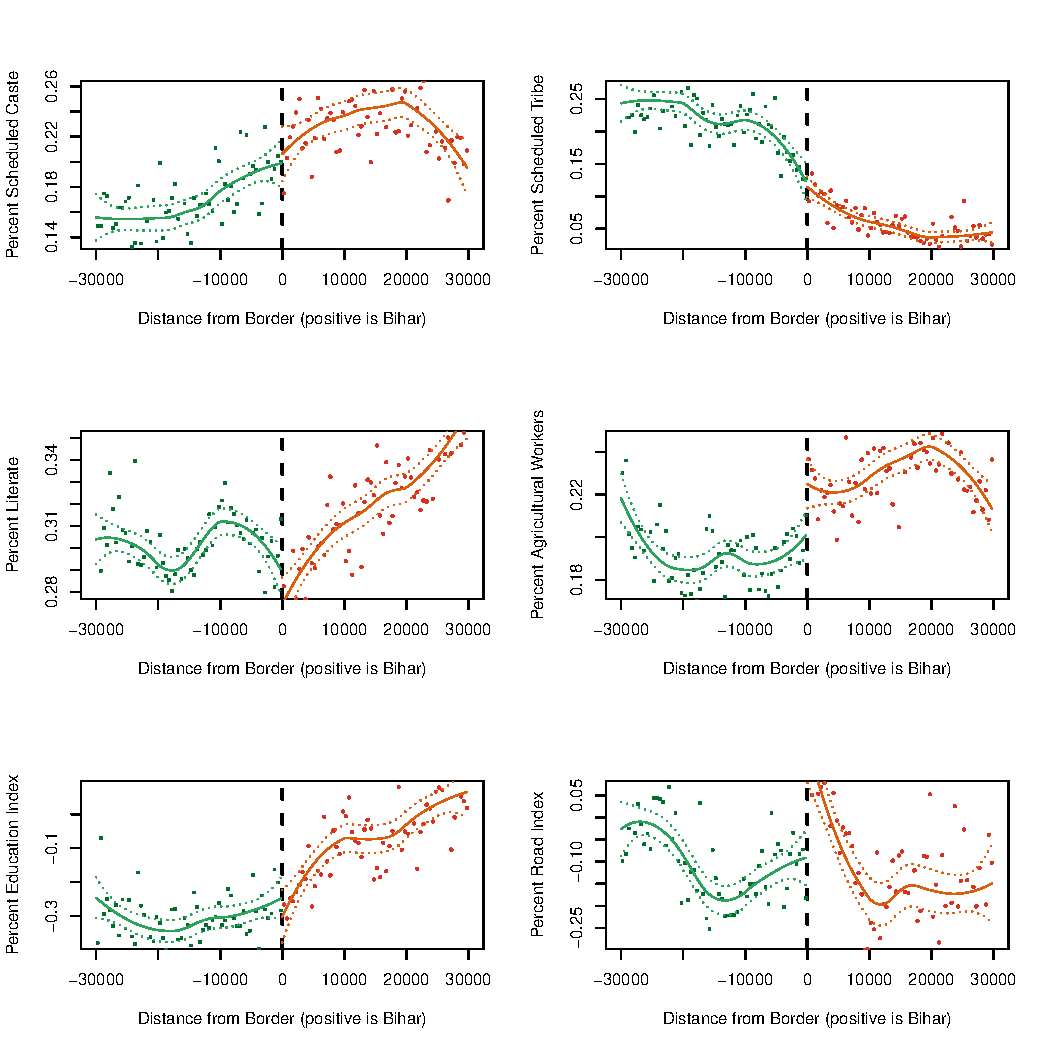
\includegraphics[width=\maxwidth]{figure/rdd_01-1.pdf}
\end{figure}
\end{frame}

\begin{frame}
\begin{figure}
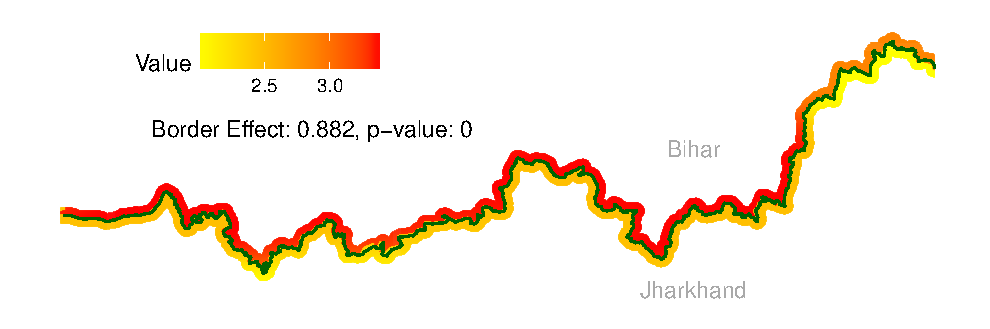
\includegraphics[width=\maxwidth]{figure/rdd_map_incumb_dist_pg-1} \caption[Predicted Value Plot of Likelihood of Incumbent Providing Public Goods if Reelected]{Predicted Value Plot of Likelihood of Incumbent Providing Public Goods if Reelected}\label{fig:rdd_map_incumb_dist_pg}
\end{figure}
\end{frame}

\begin{frame}
\begin{figure}
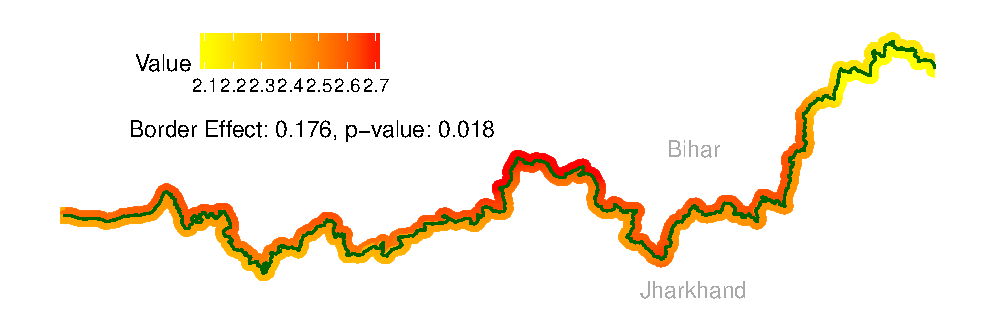
\includegraphics[width=\maxwidth]{figure/rdd_map_accountability_elite-1} \caption[Predicted Value Plot of Likelihood of Corrupt Elite being Caught]{Predicted Value Plot of Likelihood of Corrupt Elite being Caught}\label{fig:rdd_map_accountability_elite}
\end{figure}
\end{frame}

\begin{frame}
\begin{figure}
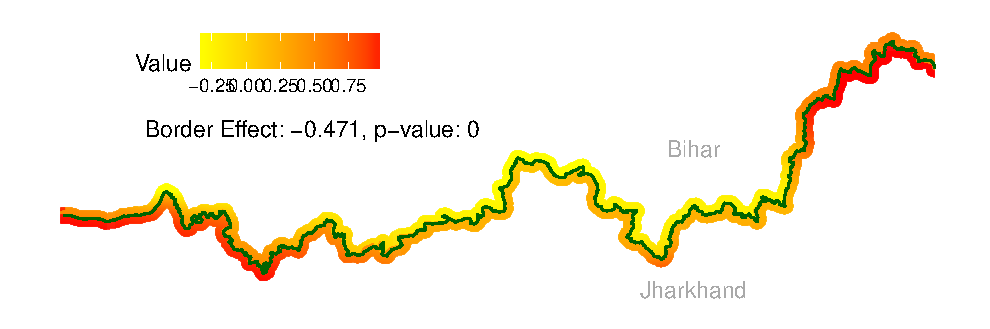
\includegraphics[width=\maxwidth]{figure/rdd_map_sabha_att-1} \caption[Predicted Value Plot of Gram Sabha Attendance]{Predicted Value Plot of Gram Sabha Attendance}\label{fig:rdd_map_sabha_att}
\end{figure}
\end{frame}

\begin{frame}
\frametitle{Geographic Discontinuities}
\begin{itemize}
\item Interpretation:
\begin{itemize}
\item Programmatic policy has changed voters' attitudes and expectations
\end{itemize}
\item But some imbalance at the border...
\pause
\item ...And compound treatment makes interpretation difficult
\end{itemize}
\end{frame}

\end{document}
